\documentclass[hyperref={pdfpagelabels=false}]{beamer}
\usepackage{lmodern}
\usepackage[utf8]{inputenc}
\usepackage{amssymb}
\usepackage{amsmath}
\usepackage{tikz}
\usepackage{tkz-euclide}
\usepackage{pifont}
\usepackage[percent]{overpic}
\usetikzlibrary{arrows,calc,intersections,shapes,backgrounds,shadows,automata}
\usetheme[compress]{Berlin}
\definecolor{UniRed}{RGB}{255,0,0}
\definecolor{UniWhite}{RGB}{255,255,255}
\definecolor{PresiBlue}{RGB}{50,57,171}
\setbeamercolor{eecks} {bg=UniRed, fg=UniWhite}
\setbeamercolor{presinative}{bg=PresiBlue, fg=UniWhite}
\newcommand{\cmark}{\ding{51}}
\newcommand{\xmark}{\ding{55}}

% Title
\title{\textsc{RoboSoccer} Project Plan}
\author[Hofbauer, Jiang, Meyer, Schmidt, Wirnshofer]{
  Markus~Hofbauer \and
  He~Jiang \and
  Kevin~Meyer \and
  Benedikt~Schmidt \and
  Florian~Wirnshofer
}
\institute
{
	Technische Universität München, Germany
}
\date{June 25, 2014}

% Presentation
\begin{document}
\begin{frame}
	\titlepage
\end{frame}

\begin{frame}
\frametitle{Countdown}
	\hfill
		\begin{beamercolorbox}[shadow=true, rounded=true, wd=10cm]{presinative}
			\centering
			\Large{\textbf{Only }}
			\Huge \color {white}{\textbf{7 Days}}
			\Large\color {white}{\textbf{are left until \newline RoSo Championship}}
		\end{beamercolorbox}
	\hfill
	\begin{figure}
		\centering
		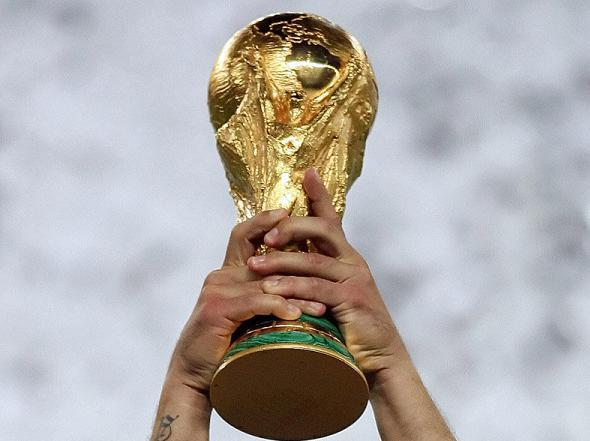
\includegraphics[width=0.6\textwidth]{Pictures/wm}
	\end{figure}
\end{frame}

\begin{frame}
	\frametitle{Table of contents}
	\tableofcontents
\end{frame}

\section{Project Progress}
\subsection{}
\begin{frame}
    \frametitle{Checklist}
    \textbf{Current Progress}
    \begin{itemize}
        \item Driving \cmark
        \begin{itemize}
            \item Controlling \cmark
            \item Collision Avoidance \cmark
        \end{itemize}
        \item Shooting \cmark
        \item Goalkeeper \cmark
        \item Referee interaction \cmark
        \begin{itemize}
            \item Connection \cmark
            \item Penalty shootout \cmark
        \end{itemize}
        \item Strategy and Tactics \xmark
    \end{itemize}
\end{frame}

\section{Strategy}
\subsection{Overview}
\begin{frame}
    \frametitle{Strategy}
    \begin{figure}
        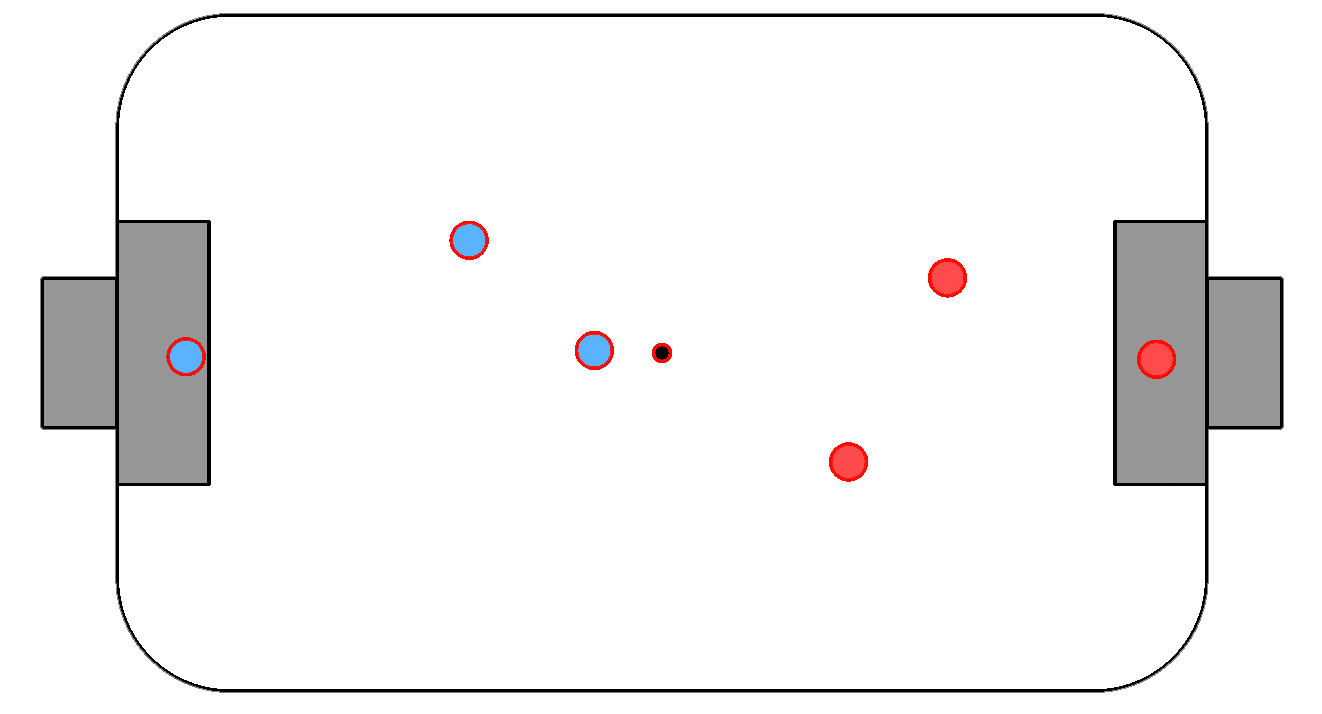
\includegraphics[width=0.7\textwidth]{Pictures/strategy}
    \end{figure}
    \textbf{Strategy:} \textit{What do we want to do?}\\
    \textbf{Tactics:} \textit{How can we achieve it?}
\end{frame}

\begin{frame}
    \frametitle{Solution}
    \textbf{Goalkeeper:}\\
    \begin{itemize}
        \item Calculate target position depending on ball position\\
        (see previous presentations)
        \item Fixed robot
    \end{itemize}

    \textbf{Field players:}\\
    \begin{itemize}
        \item \textbf{One} strategy for both field players
        \item \textbf{Small} binary decision tree
        \item Recalculated each iteration
        \item Depending on ball and robot positions
    \end{itemize}

\end{frame}

\subsection{Solution}
\begin{frame}
    \frametitle{Decision Tree}
    \begin{center}
        %!tikz editor 1.0
%!tikz source begin
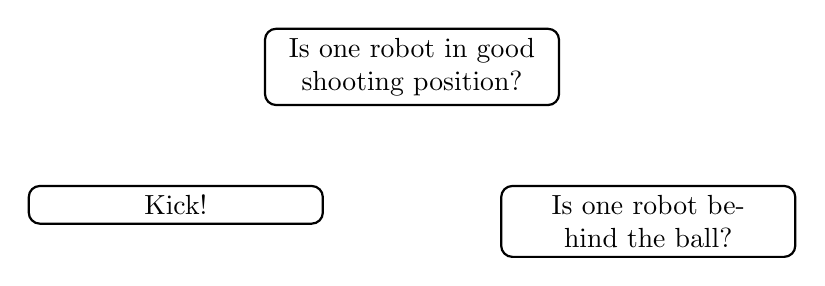
\begin{tikzpicture}
	\font\btt=rm-lmtk10
	\definecolor{PresiBlue}{RGB}{50,57,171}
	
	\tikzstyle{class}=[
		rectangle, draw=black, rounded corners, 
		text centered, anchor=north, text=black, text width=3.5cm, thick]

	\node (isgoodkickposition) [class] {Is one robot in good shooting position?};
	\node (kick) [class, below = of isgoodkickposition, xshift=-3.0cm]{Kick!};

	\node (isbehindball) [class, below = of isgoodkickposition, xshift=3.0cm]{Is one robot behind the ball?};
	
\end{tikzpicture}
%!tikz source end

    \end{center}
\end{frame}

\subsection{Implementation}
\begin{frame}
    \frametitle{Class Diagramm}
    \begin{center}
        %!tikz editor 1.0
%!tikz source begin
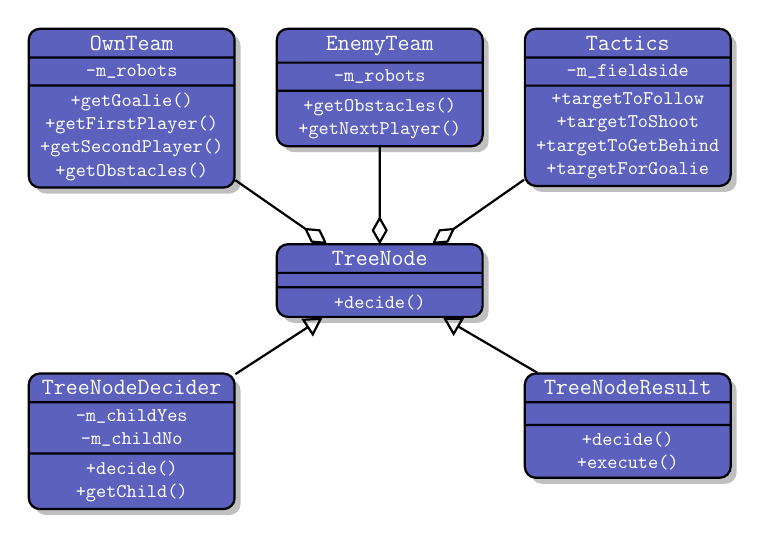
\begin{tikzpicture}[node distance=4.5cm, scale=0.7, transform shape]
	\font\btt=rm-lmtk10
	\definecolor{PresiBlue}{RGB}{50,57,171}
	
	\tikzstyle{class}=[
		rectangle, draw=black, rounded corners, rectangle split, rectangle split parts=3, 
		fill=PresiBlue!80, drop shadow, font=\tt,
        text centered, anchor=north, text=white, text width=3.5cm, thick]
		
	\tikzstyle{inheritance}=[draw, ->, >=open triangle 60, thick]
	\tikzstyle{property}=[draw, ->, >=open diamond, thick]
	\tikzstyle{line}=[-, thick]
   
   % Classes
      
	\node (treenode) [class]
	{
		{\large \texttt{\textbf{TreeNode}}}
		
		\nodepart{second}
		
		\nodepart{third}
		+decide()
	};
	
	\node (treenodedecider) [class, left =of treenode.south, anchor = north, yshift=-1cm]
	{
		{\large \texttt{\textbf{TreeNodeDecider}}}
		
		\nodepart{second}
		-m\char`_childYes\\
		-m\char`_childNo
		
		\nodepart{third}
		+decide()\\
		+getChild()
	} edge [inheritance] (treenode);
	
	\node (treenoderesult) [class, right =of treenode.south, anchor = north, yshift=-1cm]
	{
		{\large \texttt{\textbf{TreeNodeResult}}}
		\nodepart{third}
		+decide()\\
		+execute()		
	} edge [inheritance] (treenode);

	\node (ownteam) [class, left = of treenode.north, anchor = south, yshift=1cm]
	{
		{\large \texttt{\textbf{OwnTeam}}}
		
		\nodepart{second}
		-m\char`_robots
		
		\nodepart{third}
		+getGoalie()\\
		+getFirstPlayer()\\
		+getSecondPlayer()\\
		+getObstacles()
		
	} edge [property] (treenode);

	\node (enemyteam) [class, right = of ownteam.north, anchor = north]
	{
		{\large \texttt{\textbf{EnemyTeam}}}

		\nodepart{second}
		-m\char`_robots
		
		\nodepart{third}
		+getObstacles()\\
		+getNextPlayer()

	} edge [property] (treenode);

	\node (tactics) [class, right = of enemyteam.north, anchor = north]
	{
		{\large \texttt{\textbf{Tactics}}}
		
		\nodepart{second}
		-m\char`_fieldside
		
		\nodepart{third}
		+targetToFollow\\
		+targetToShoot\\
		+targetToGetBehind\\
		+targetForGoalie
	} edge [property] (treenode);


	% Connections
	
	
\end{tikzpicture}
%!tikz source end

    \end{center}
\end{frame}

\section{GUI Tool}
\subsection{}
\begin{frame}
    \frametitle{Validation GUI}
    \begin{figure}
        \center
        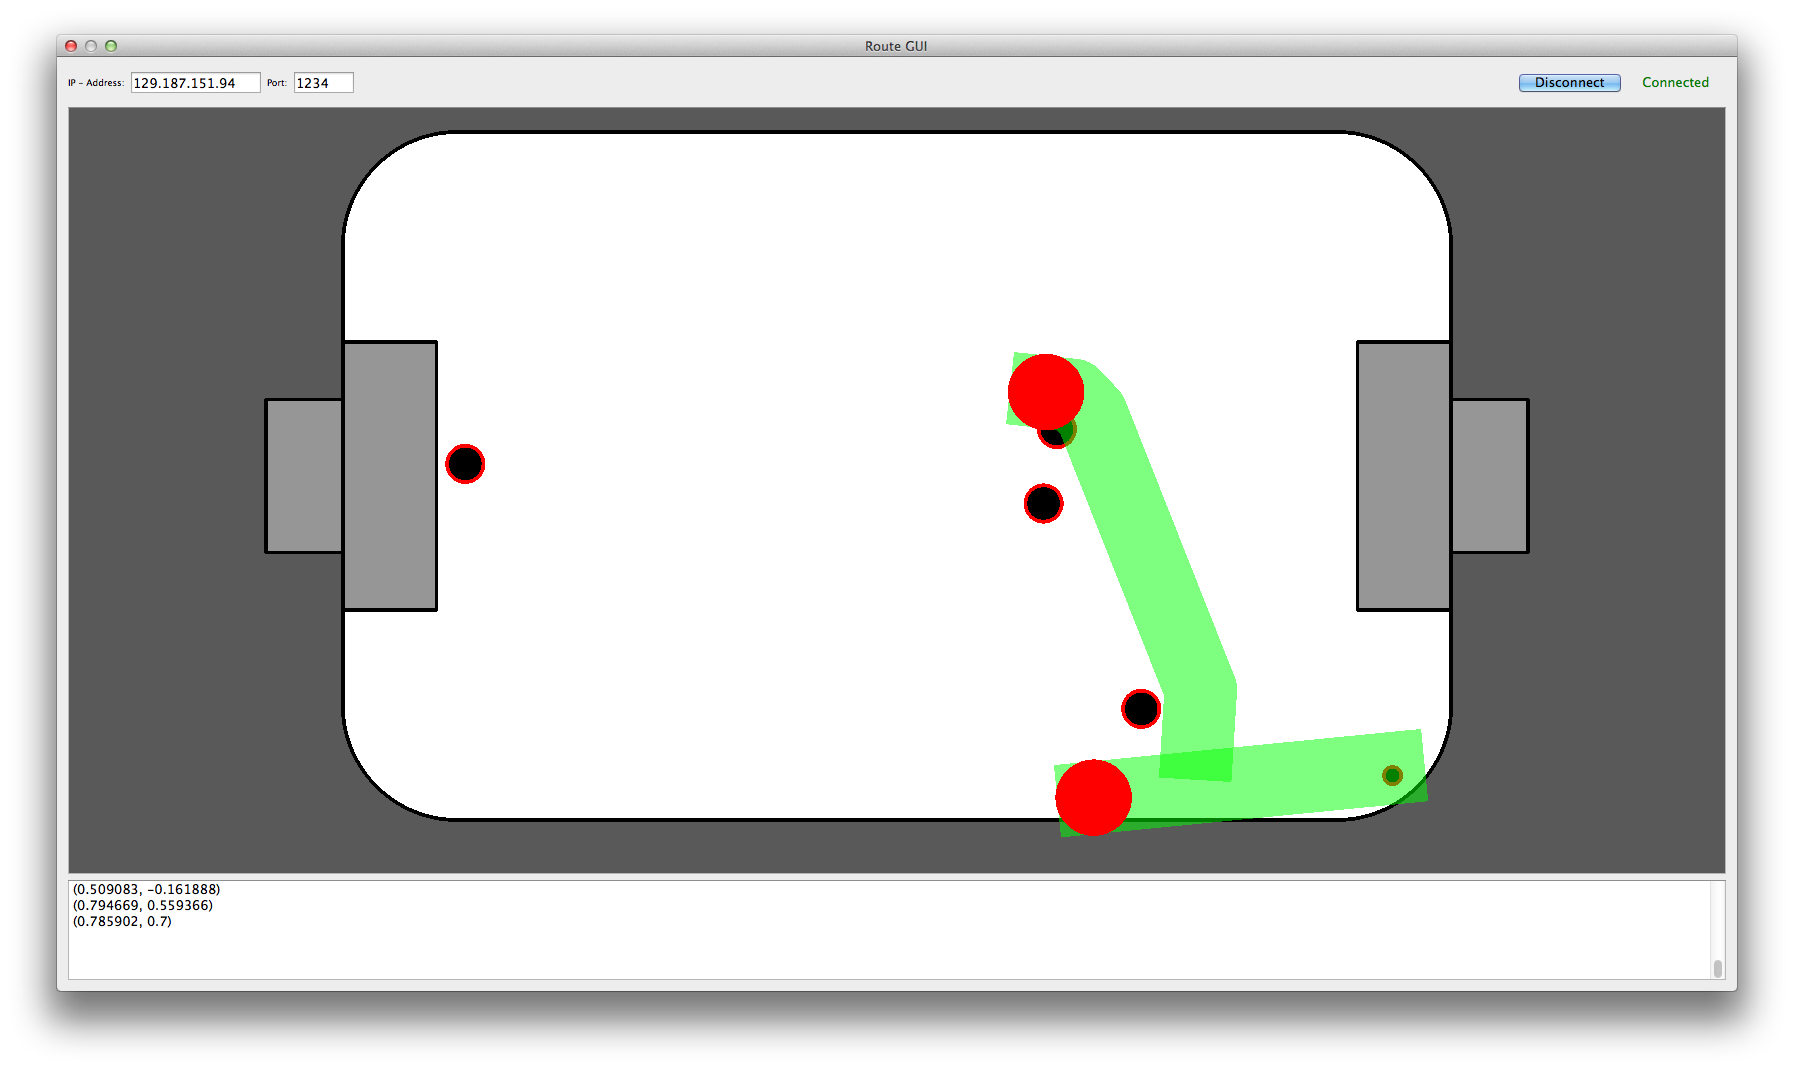
\includegraphics[width=0.95\textwidth]{Pictures/gui-big}
    \end{figure}

\end{frame}

\begin{frame}
    \frametitle{Validation GUI}
    \begin{columns}[T]
        \begin{column}{0.4\textwidth}
            \begin{figure}
                \center
                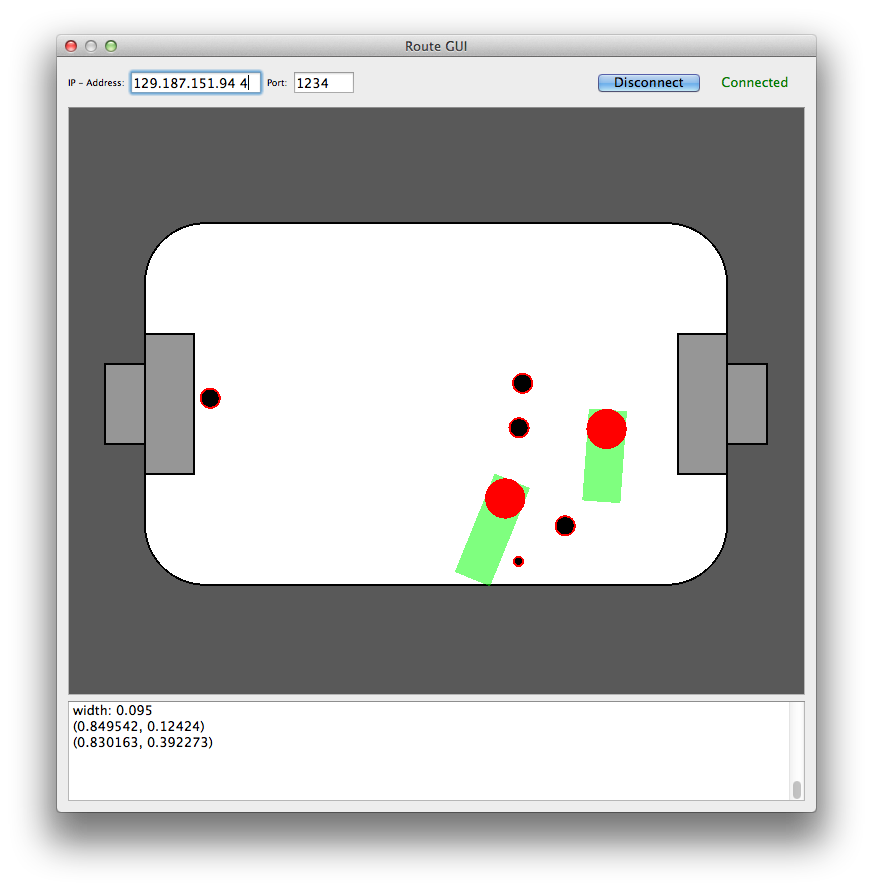
\includegraphics[width=\textwidth]{Pictures/gui-small}
            \end{figure}
        \end{column}
        \begin{column}{0.6\textwidth}
            \textbf{Features:}
            \begin{itemize}
                \item Connects via \textbf{network}
                \item Updates \textbf{live and in realtime}
                \item Shows own robots and \textbf{routes}
                \item Displays all obstacles
                \item Logs positions
            \end{itemize}
        \end{column}
    \end{columns}
\end{frame}

\begin{frame}
    \frametitle{Validation GUI}
    \begin{columns}[T]
        \begin{column}{0.4\textwidth}
            \begin{figure}
                \center
                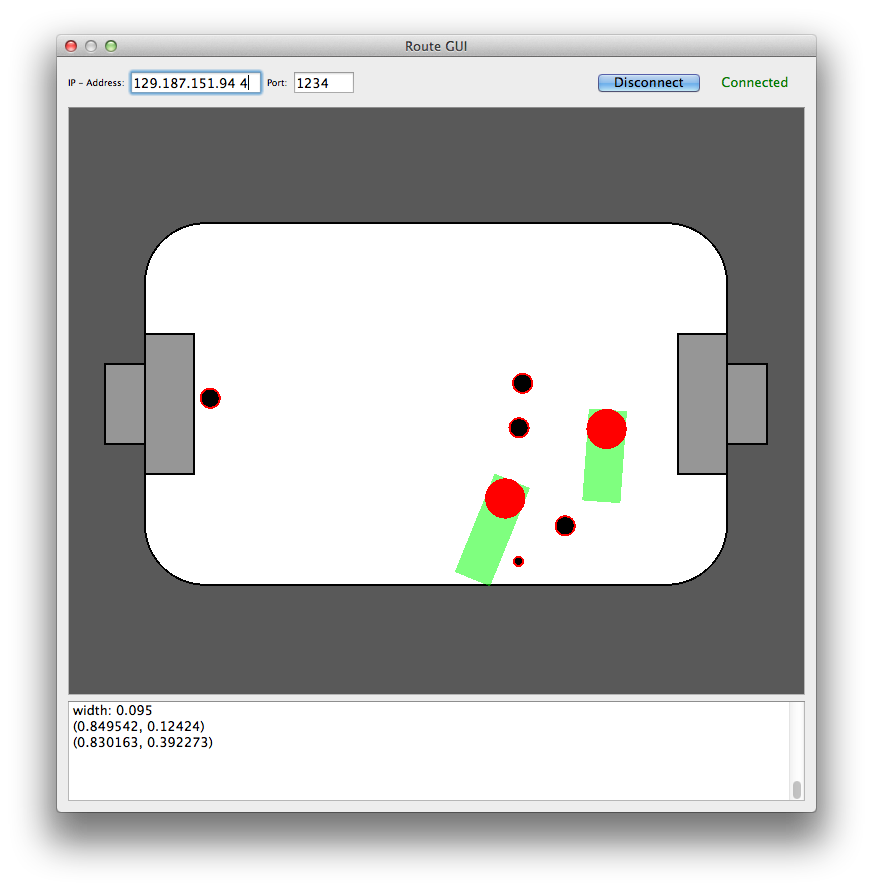
\includegraphics[width=\textwidth]{Pictures/gui-small}
            \end{figure}
        \end{column}
        \begin{column}{0.6\textwidth}
            \textbf{Implementation:}
            \begin{itemize}
                \item Seperate \textsc{Qt 5} project
                \item Connection via TCP/IP Socket
                \item Drawing on \textsc{QGraphicsView}
            \end{itemize}
        \end{column}
    \end{columns}
\end{frame}

\begin{frame}
    \frametitle{Validation GUI}
    \begin{columns}[T]
        \begin{column}{0.4\textwidth}
            \begin{figure}
                \center
                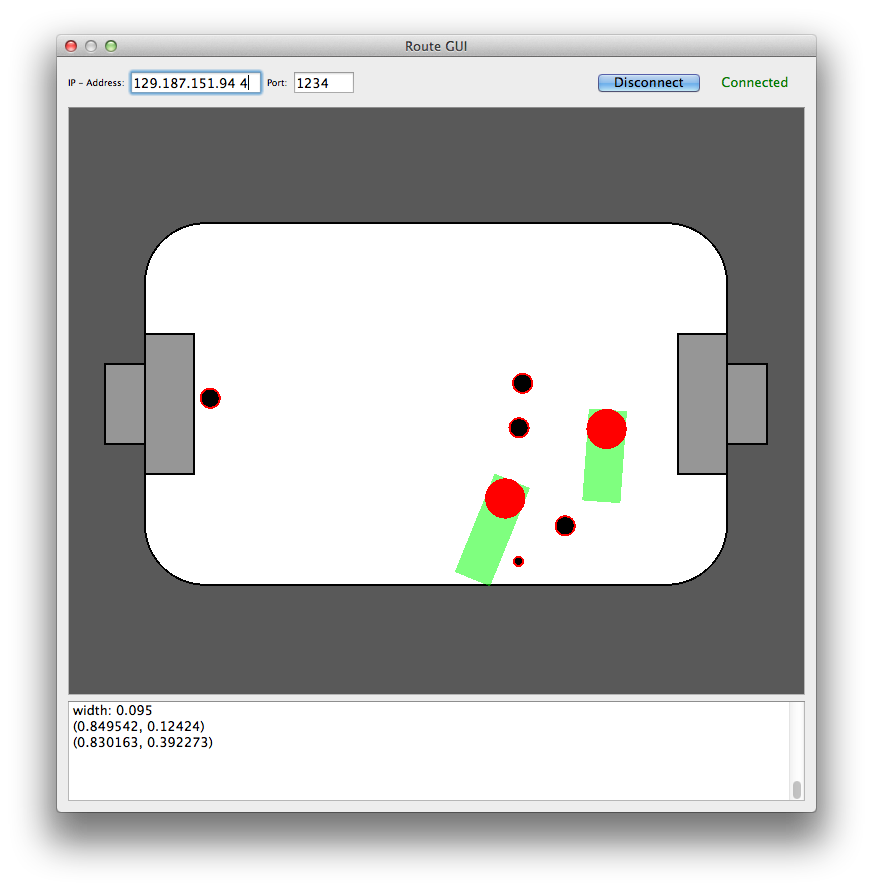
\includegraphics[width=\textwidth]{Pictures/gui-small}
            \end{figure}
        \end{column}
        \begin{column}{0.6\textwidth}
            \begin{minipage}[c][.57\textheight][c]{\linewidth}
                \begin{center}
                    \textbf{\textit{\Large Demo?}}\\
                    $\rightarrow$ Later in the laboratory
                \end{center}
            \end{minipage}
        \end{column}
    \end{columns}
\end{frame}

\section{Schedule}
\subsection{}
\section{Gantt Chart}
\begin{frame}
	\frametitle{Gantt Chart}
	\begin{figure}
		\centering
		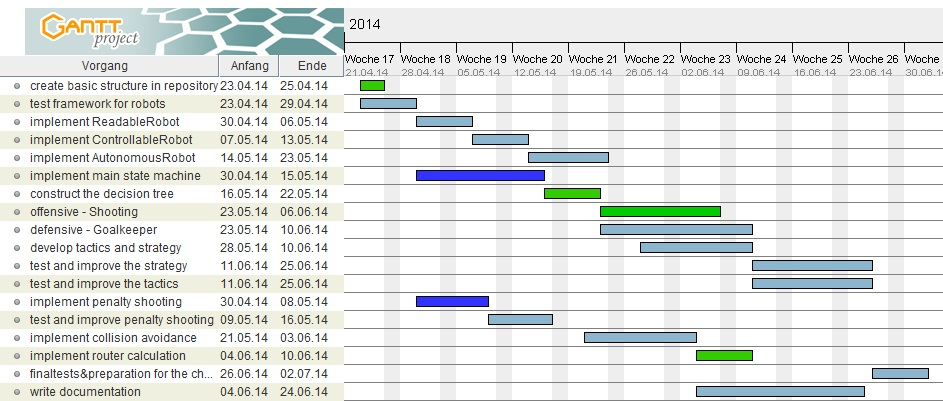
\includegraphics[width=0.95\textwidth]{Pictures/gantt1}
	\end{figure}
\end{frame}

\section{}
\begin{frame}
	\hfill
	\begin{beamercolorbox}[shadow=true, rounded=true, wd=10cm]{presinative}
		\centering
		\Large{\textbf{Thank you for your attention!}}
	\end{beamercolorbox}
	\hfill
\end{frame}

\end{document}
